\documentclass[a4paper,11pt]{article}
\usepackage[margin=1.5cm]{geometry}
\usepackage{amsmath}
\usepackage{amssymb}
\usepackage{color}
\usepackage{graphicx}
\usepackage{graphics}
\usepackage[margin=1.5cm]{geometry}
\usepackage{fancyhdr}
\usepackage{float}
\usepackage{wrapfig}
\usepackage{lscape}
\usepackage[font={small},labelfont=bf]{caption}
\usepackage[usenames,dvipsnames,svgnames,table]{xcolor}

\bibliographystyle{unsrt}
%\linespread{1.2}

%%%%%%%
%Defines vectors universally, for ease of editing and consistency.
\newcommand{\vtr}[1] {\mathit{\underline{\boldsymbol{#1}}}}

%Draws a big red box containing the text as in \ALERT{<TEXT HERE>}. For labelling draft copies with important notes.
\def\ALERT#1{\begin{center}\colorbox{red}{\hbox{\textcolor{black}{\textbf{#1}}}}\end{center}}

%Roman-style subscript; removes math-mode font.
\def\s#1{_\textrm{#1} }

%The operators in integrals and derivatives.
\def\d{\operatorname{d}\!}

%The Euler e should be in Roman font.
\def\e{\textrm{e}}

%%%%%%%%%%%   some definitions used in latexing the CQMP:
% fractions that are of right size in set equations
\def\half{{\textstyle \frac{1}{2}}}
\def\quarter{{\textstyle \frac{1}{4}}}
\def\third{{\textstyle \frac{1}{3}}}
\def\eighth{{\textstyle \frac{1}{8}}}

% obtain a new line
\def\nl{\hfil\break}
%%%%%%%%%

\title{Physical Concept: \textbf{Friction}}
%\author{Mark Warner}
\date{}

%******************************* to optimise page usage
\setlength{\textwidth}{6.3 in}

\setlength{\oddsidemargin}{0.2 in}
\setlength{\evensidemargin}{0.2 in}

\setlength{\topmargin}{-.80 in}
\setlength{\textheight}{9.9 in}
%*******************************

% to mark as a draft.  Comment both these lines out when complete.  The page number will return to the footer.
%\pagestyle{myheadings}
%\markright{\textcolor{red}{\textbf{DRAFT: \today}}}


\begin{document}
%\vspace{-5cm}
%\maketitle
\noindent
{\huge Physical Concept: \textbf{Friction}}
%\vspace{1cm}
%\nl
%{\bf Circular kinematics}
%\nl
%\vspace{-2cm}
\section{Definitions}
\begin{wrapfigure}{r}{6cm}\vspace{-1cm}
\center
\includegraphics[width=0.35\textwidth]{friction-defs.eps}
\caption{A block sitting \textit{at rest }on a rough plane.  The weight has an equilibrant $\vtr{R} = - m\vtr{g}$ acting on it from the plane.  An applied force $\vtr{F}$ is resisted by a frictional force $\vtr{F}_f = -\vtr{F}$ from the plane acting on the block.  The plane in turn has the frictional reaction force $-\vtr{F}_f$ acting on it from the block.}
\label{fig:friction-defs}
\end{wrapfigure}
\vspace{-.3cm}
Figure~\ref{fig:friction-defs} shows a block of mass $m$ sitting at rest on a rough plane. The weight, reaction, applied and frictional forces are shown.  The frictional force is of magnitude $F_f = F$ equal to the applied force so the block does not move horizontally.  By Coulomb's law of friction:
 \begin{equation*} F_f  \le \mu R
\end{equation*}
where $\mu$ is the coefficient of static friction and depends on the character of the two surfaces in contact, but \textit{not} their area.  It does not have units since it is a ratio $F_f/R$ of forces.
%\begin{table*}[!h]\caption{Selected static and kinetic coefficients of friction.}
\begin{wrapfigure}{r}{7cm}\vspace{-0.5cm}
%\begin{centering}
  \begin{tabular}{|c|c|c|c|}
\hline
Material & Material & $\mu$ & $\mu_k$\\
\hline
\hline
   Wood & Leather &$0.61$& 0.52 \\
   \hline
   Ice & Steel &0.03& \\
    \hline
   Horse shoe   & Concrete &0.58& \\
 \hline
   Rubber & Asphalt &0.9&0.5 \\
   \hline

  \end{tabular}
%\end{centering}%\\
 % \end{table*}
\end{wrapfigure}
When the applied force exceeds $\mu R$, then the block starts to slide.  The frictional force is now $F_f = \mu_k R$ where $\mu_k$ is the coefficient of sliding, dynamic or kinetic friction.  Clearly $\mu_k < \mu$, so once sliding starts under the influence of an applied force, then the resistive effect of the frictional contact between the surfaces is reduced.

Typical values of $\mu$ are given in the table.\\
\begin{wrapfigure}{r}{7cm}\vspace{-1cm}
\center
\includegraphics[width=0.35\textwidth]{slope.eps}
\caption{A rough slope inclined at angle $\theta$ to the horizontal with a block of mass $m$ resting on it.  The vector triangle resolves the weight force parallel and perpendicular to the slope.}
\label{fig:slope}
\end{wrapfigure}

\section{Examples}
\vspace{-.3cm}
  Q1.   A rough slope with a coefficient of friction $\mu$ with a block makes an angle $\theta$ with the horizontal.  At what angle does a block resting on the surface start slipping?\\

From the vector triangle of figure~\ref{fig:slope}, one sees that the normal component of the weight force into the surface is of magnitude $mg\cos\theta$ which is also the value of the reaction force $R$.  Hence the maximum frictional resistive force acting up the slope on the block is $F_f = \mu mg \cos\theta$.  The component of weight down the slope is $mg\sin\theta$.  At the maximal angle before slipping, this downwards component is exactly balanced by the frictional force, that is
\begin{equation*} mg\sin\theta = \mu mg \cos\theta \rightarrow \tan\theta = \mu
\end{equation*}
on cancelling  $mg$ on each side and dividing through by $\cos\theta$.\\
  Q2.  If the angle becomes such that the block starts sliding, to what value must $\theta$ be reduced to stop it sliding?  [Answer: $\theta = \arctan(\mu_k)$.]\\
  Q3. Harder* If the block just starts sliding and the slope is not reduced, what is the acceleration of the block down the slope? [Answer: $a = g(\mu -\mu_k)/\sqrt{1 + \mu^2}$.]\\
  \vspace{.4cm}
  
  \noindent
{\large \textbf{Friction \& Rolling}}\\
For cylinders and spheres to roll rather than skid, frictional contact with their support surface is required.  Once rolling is achieved the frictional force, acting at the point of contact, is not a moving force and does no work.  Friction determines the dynamics without causing energy loss.
\end{document}
